\pagenumbering{arabic}
\section{概述}

\subsection{简述}

数字电子钟是一种用数字显示秒、分、时、日的计时装置,与传统的机械钟相比,它具有走时准确,显示直观、无机械传动装置等优点,因而得到了广泛的应用。小到人们日常生活中的电子手表,大到车站、码头、机场等公共场所的大型数显电子钟。

数字电子钟由以下几部分组成:石英晶体振荡器和分频器组成的秒脉冲发生器;校时电路;六十进制秒、分计数器,二十四进制(或十二进制)计时计数器;秒、分、时的译码显示部分等。


\subsection{设计任务和要求}

用中、小规模集成电路设计一台能显示日、时、分、秒的数字电子钟,要求如下:

\begin{enumerate}[1.]
\item 由晶振电路产生1Hz标准秒信号。
\item 秒、分为00~59六十进制计数器。
\item 时为00~23二十四进制计数器。
\item 周显示从1~日为七进制计数器。
\item 可手动校时:能分别进行秒、分、时、日的校时。只要将开关置于手动位置,可分别对秒、分、时、日进行手动脉冲输入调整或连续脉冲输入的校正。
\item 整点报时。整点报时电路要求在每个整点前呜叫五次低音(500Hz),整点时再呜叫一次高音(1000Hz)。
\end{enumerate}

\subsection{设计工具}

\begin{itemize}
	\item Multisim 14.0(电路仿真)
	\item LaTeX(文档编写)
	\item OBS+格式工厂(功能演示视频录制)
	\item Visio 2016(流程图绘制)
\end{itemize}

\subsection{元件清单}

74 系列的元件有以下几种,在我的设计中用的的元件清单如表 \ref{tool} 所示。

\begin{enumerate}[1)]
	\item 74××(标准型)
	\item 74S××(肖特基)
	\item 74LS××(低功耗肖特基)
	\item 74ALS××(先进低功耗肖特基)
	\item 74AS××(先进肖特基)
	\item 74F××(高速)
\end{enumerate}


\begin{table}[hbtp]
	\setlength{\abovecaptionskip}{0cm} 
	\setlength{\belowcaptionskip}{-0.2cm}
	\begin{center}
	\caption{元件清单表}
	\begin{tabular}{|c|p{4cm}<{\centering}|p{2cm}<{\centering}|c|c|}
		\hline
		\textbf{Quantity} & \textbf{Description}  & \textbf{RefDes}               & \textbf{Package}                   & \textbf{Obsolete} \\ \hline
		1                 & TIMER, LM555CM        & U1                            & IPC-7351\textbackslash{}M08A       & No                \\ \hline
		7                 & 74STD, 74160N         & U2, U3, U7, U8, U12, U13, U17 & IPC-2221A/2222\textbackslash{}NO16 & No                \\ \hline
		3                 & 74STD, 7410N          & U6, U11, U16                  & IPC-2221A/2222\textbackslash{}NO14 & No                \\ \hline
		1                 & 74STD, 7427N          & U20                           & IPC-2221A/2222\textbackslash{}NO14 & No                \\ \hline
		4                 & 74STD, 7400N          & U19, U21, U22, U23            & IPC-2221A/2222\textbackslash{}NO14 & No                \\ \hline
		3                 & SPDT,                 & S1, S2, S3                    & Generic\textbackslash{}SPDT        & -                 \\ \hline
		3                 & 74STD, 7451N          & U24, U25, U28                 & IPC-2221A/2222\textbackslash{}NO14 & No                \\ \hline
		4                 & 74STD, 7404N          & U26, U27, U29, U31            & IPC-2221A/2222\textbackslash{}NO14 & No                \\ \hline
		1                 & BUZZER, BUZZER 500Hz  & LS1                           & Generic\textbackslash{}BUZZER      & -                 \\ \hline
		1                 & 74STD, 7408N          & U34                           & IPC-2221A/2222\textbackslash{}NO14 & No                \\ \hline
		1                 & BUZZER, BUZZER 1000Hz & LS2                           & Generic\textbackslash{}BUZZER      & -                 \\ \hline
	\end{tabular} \label{tool}
	\end{center}
\end{table}

\subsection{设计方案流程图}

数字电子钟设计的流程图如图 \ref{fig:FlowChart} 所示。


\begin{figure}[hbtp]
	\centering
	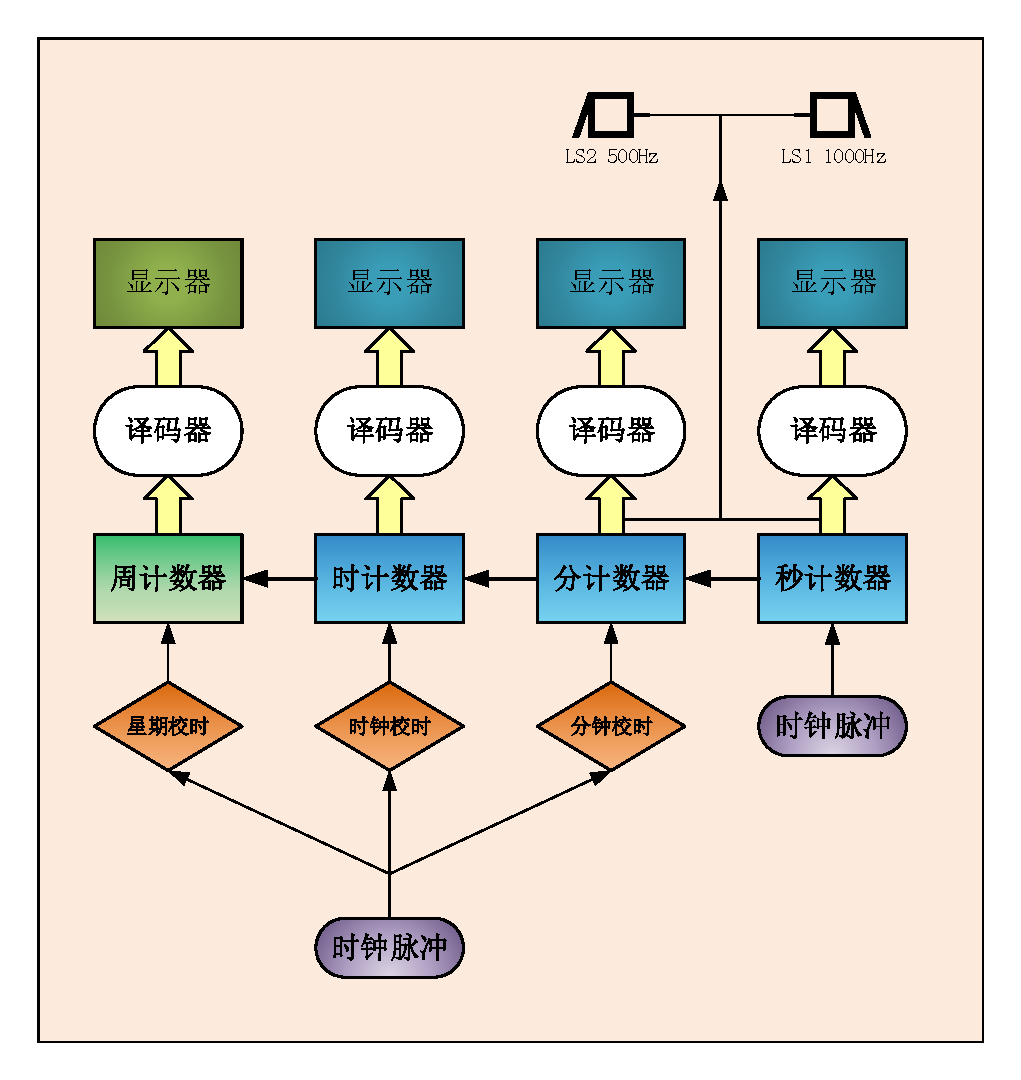
\includegraphics[width=16cm]{figure/FlowChart}
	\caption{设计流程图}\label{fig:FlowChart}
\end{figure}